\documentclass[a4paper]{article}

\usepackage[fancy]{template}
\usepackage{survival-pack}

\setup{%
  subject={Datanet},%
  assignment={Assignment 1},%
  date={29 April, 2013}%
}
\setupLocation[short=DIKU]{Datalogisk institut, Københavns Universitet}
\setupAuthor[addendum={\email{jonas.brunsgaard@gmail.com}}]{Jonas Brunsgaard}

\newcommand{\commandstyle}[0]{{\ttfamily\textbackslash}}
\newcommand{\command}[1]{\texttt{\textbackslash #1}}

\begin{document}

\maketitle
\thispagestyle{first}
\newpage

\section{Theoretical part}
\subsection{Store and Forward}
\subsubsection{Processing and delay}
In addition to propogation delay we have

\begin{description}
    \item[Processing delay] A delay caused by the routers in the network,
        due to the requirement of examining the packet's header information to
        determine where to direct the package.
    \item[Queue delay] If more packets are going into the same link, the
        router forms a queue, where a packet is hold until it is
        transmitted, this delay is called a queue delay.
    \item[Tranmission delay] The time required to push all of the packet's bits
        into the link. This is often the most most significant delay.
\end{description}

% Calculations for the subsection on transmission speed
\subsubsection{Transmission speed}
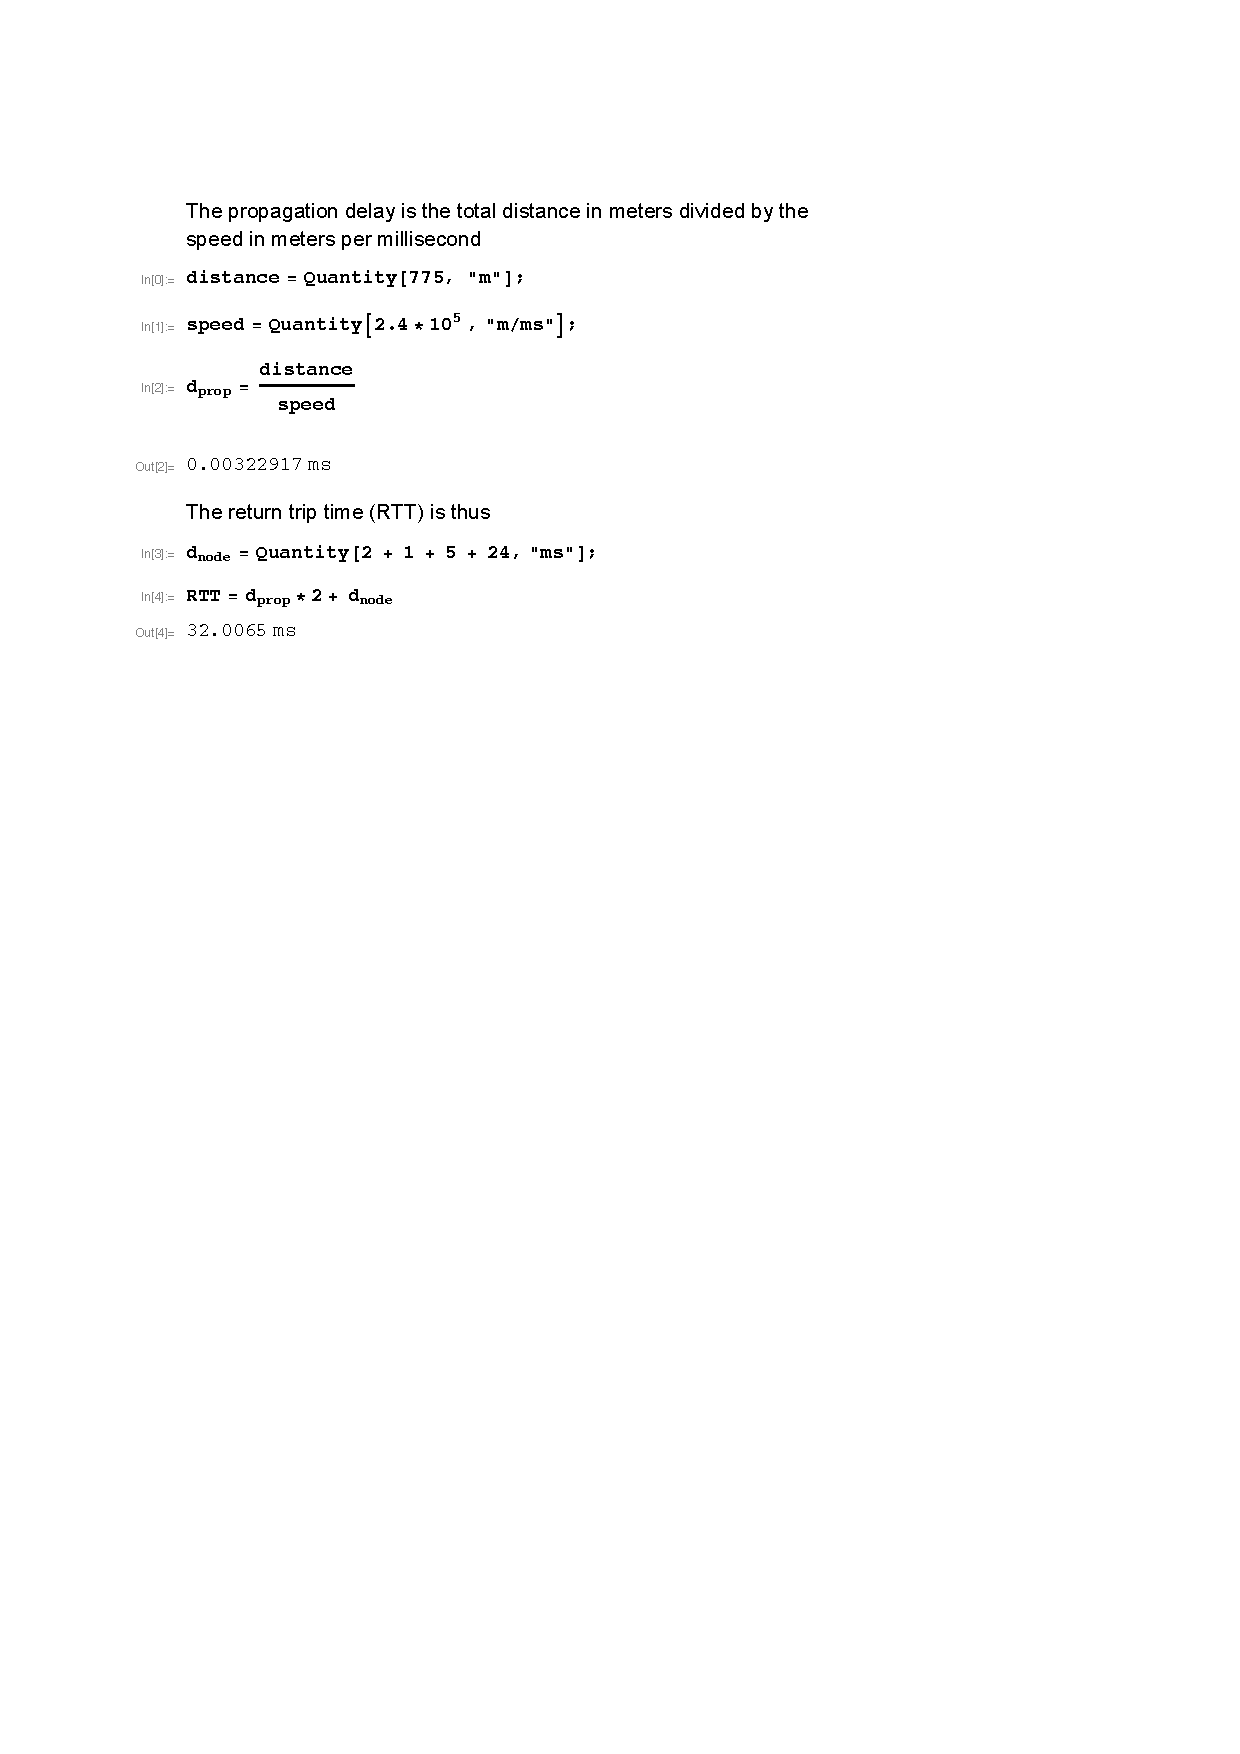
\includegraphics{../calc1.pdf}
\newpage
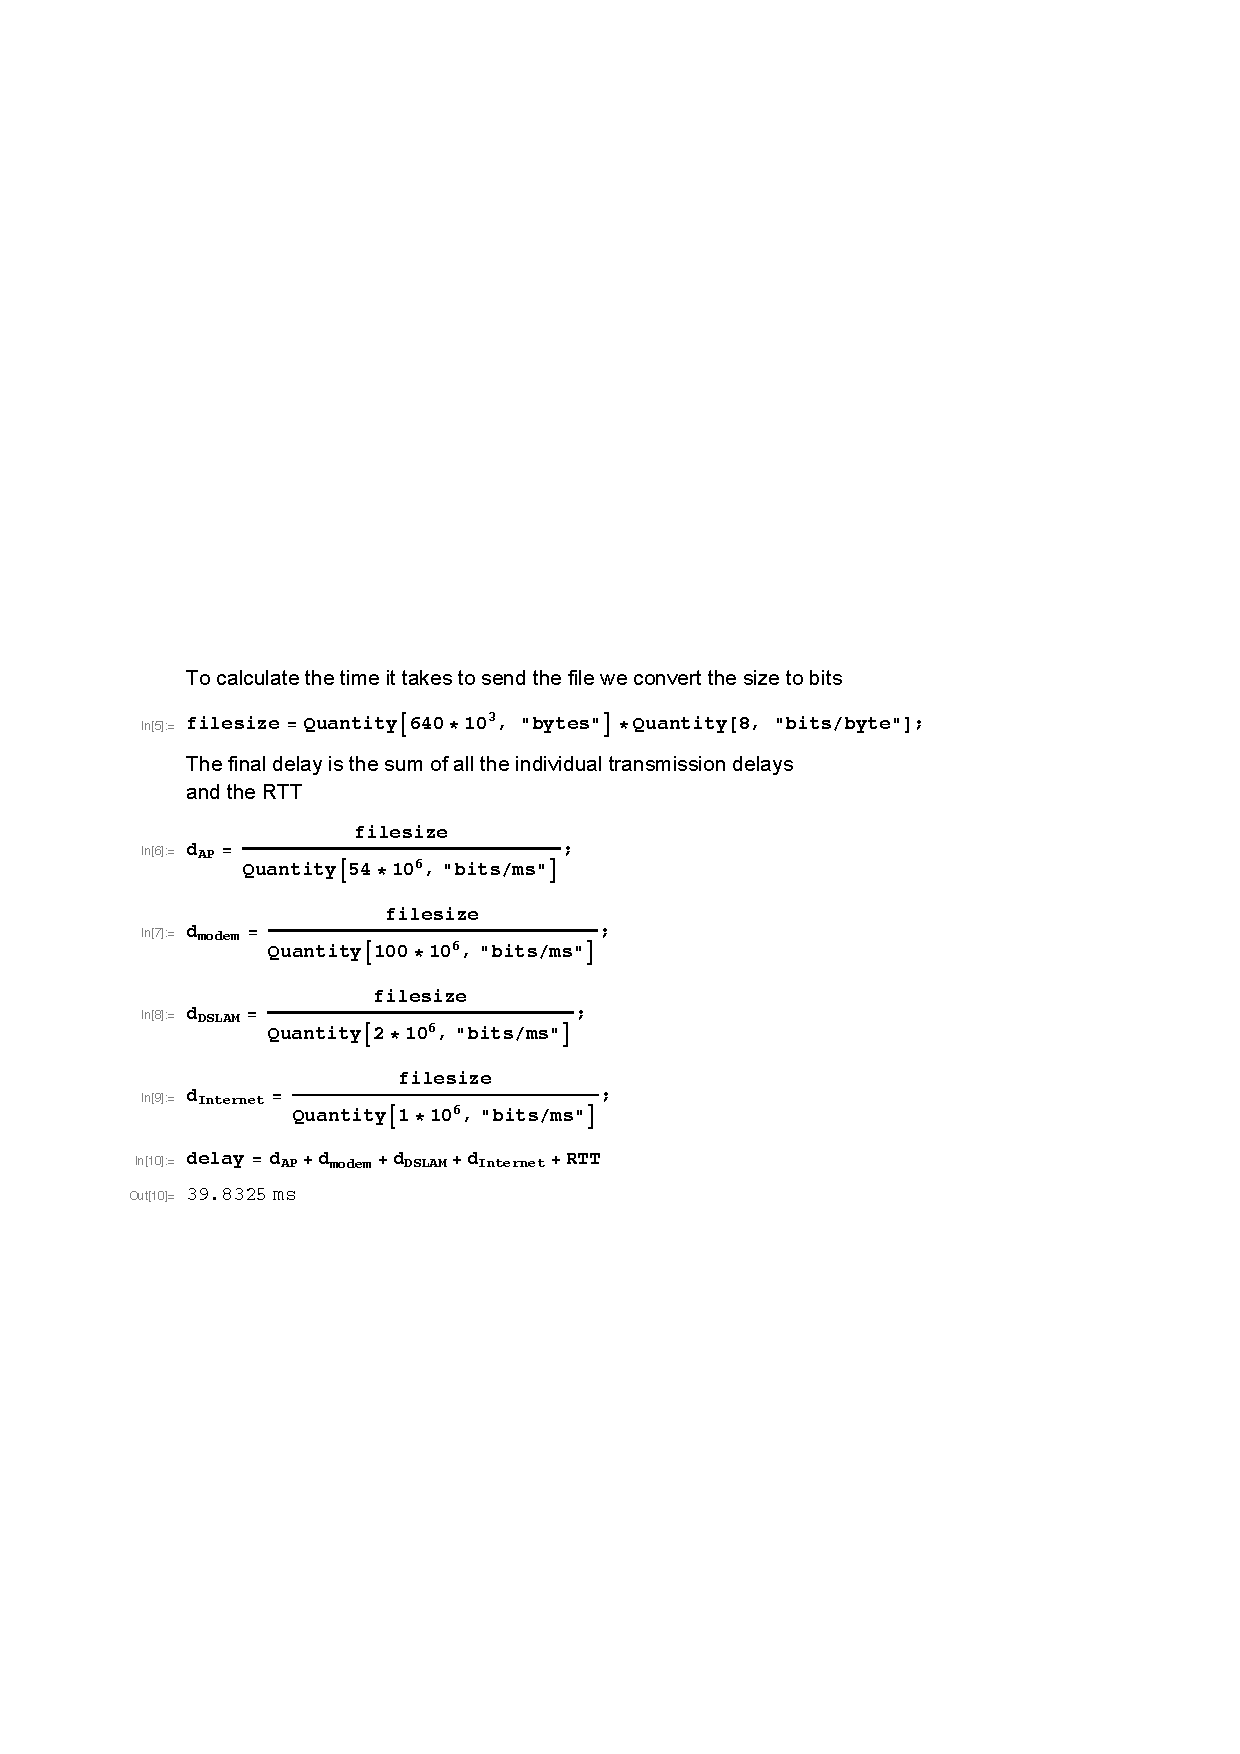
\includegraphics{../calc2.pdf}

\subsection{Buffers and latency}
\begin{description}
    \item[Part 1] The link behind the DSL modem is limited to 54 Mb/s by the wireless connection,
        but is significantly faster than the 2Mb/s upload speed of the modem. Given a continuous
        upload burst it will be filled in approx. 78.7 milliseconds, leading to further packets being
        dropped. This results in a maximum packet delay that is infinite. All packets from the student
        will then be discarded.
    \item[Part 2] The \emph{Bandwith-delay product} can be seen as a measurement of the
        ``volume'' of the network link, describing how much data that can be on the link at
        any point in time.
        TODO: Why good measure, and what are consequences?
\end{description}

\subsection{HTTP}
\subsubsection{HTTP semantics}
\subsubsection{HTTP headers and fingerprinting}

\subsubsection{The case of Deep Packet Inspection}
\begin{description}
    \item[Part 1] '3' could have filtered all requests to \texttt{grooveshark.com} by dropping all packets
        with a destination host being an IP belonging to that domain. This could be done in the network layer without
        breaking the layering model of the network stack.
    \item[Part 2] This is a violation of layering in networks because a layer is inspecting and modifying
        the data passing in a layer above it. To stop this and enforce the layering we may encrypt the HTTP
        stream by using HTTPS (SSL).
\end{description}


\section{Practical part}
\subsection{Socket Programming}

\subsubsection{Question 1}

Restricting the messages size to \texttt{BUFFER\_SIZE}, simplifies receiving data, as one only need to have a buffer of the specified size. But it also puts a strict limit on the amount of data that can be sent.
If one should take the token based approach, a good candidate for the token could be the \texttt{EOT} character, (ASCII number 4), meaning ``end of transmission''.
Using a specific buffer size is required by the socket API, so one would need to use a combination of the two. If the last character recieved is not the token for end of message, one simply recieve data once more. Each part of the message then needs to be concatenated in the end to look at the whole message.
For this particular case, limiting message size to 1024 should not be a big problem, as message sizes should be fairly small -- with the exception that one can make arbitrability large ECHO commands.

\subsubsection{Question 2}

As the protocol is stateless, as described below, we can just close the socket on the server. In our implementation the client program is terminated if the socket dies, so the client has to reconnect anyway.

\subsubsection{Question 3}

Each command in the protocol was manually tested to verify expected behavior. Both client and server handles malformed requests,
by only reacting on the specified commands. To increase robustness, clients can handle situations where the server is not up
or crashes within a session. The client does not handle malformed responses, it just prints whatever it gets.

To increase the robustness of the server one might adopt a threaded architecture, where every connecting client gets their own thread.
This could also enable several users to connect to the server in parallel. A crash in one thread would then kill the thread, but not
interfere with the working of the other threads.

The client could be crashed by sending responses containing control bytes back to the client. One might filter all the bytes that
the client receives and only display those that are in a whitelist. However this change changes the output on the client side, and
is arguably a violation of the lack of restrictions on messages that the protocol handles.

TODO: other basic steps?

\subsubsection{Question 4}

The protocol is stateless, because the server does not need to maintain any information about the client. In our implementation we keep the socket open, but the protocol does not require us to do so.


\end{document}
